% This file was created with tikzplotlib v0.10.1.
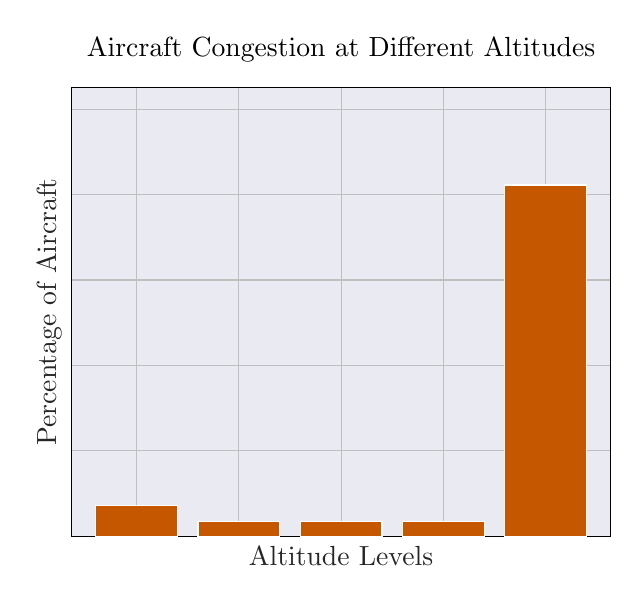
\begin{tikzpicture}

\definecolor{chocolate197870}{RGB}{197,87,0}
\definecolor{darkslategray38}{RGB}{38,38,38}
\definecolor{lavender234234242}{RGB}{234,234,242}

\begin{axis}[
axis background/.style={fill=lavender234234242},
tick align=outside,
title={Aircraft Congestion at Different Altitudes},
xlabel=\textcolor{darkslategray38}{Altitude Levels},
xmajorgrids,
xmajorticks=false,
xmin=-0.64, xmax=4.64,
xtick style={color=darkslategray38},
ylabel=\textcolor{darkslategray38}{Percentage of Aircraft},
ymajorgrids,
ymajorticks=false,
ymin=0, ymax=1.05,
ytick style={color=darkslategray38}
]
\draw[draw=white,fill=chocolate197870] (axis cs:-0.4,0) rectangle (axis cs:0.4,0.0724682404978656);
\draw[draw=white,fill=chocolate197870] (axis cs:0.6,0) rectangle (axis cs:1.4,0.0349225942498586);
\draw[draw=white,fill=chocolate197870] (axis cs:1.6,0) rectangle (axis cs:2.4,0.0349225942498586);
\draw[draw=white,fill=chocolate197870] (axis cs:2.6,0) rectangle (axis cs:3.4,0.0350768914262202);
\draw[draw=white,fill=chocolate197870] (axis cs:3.6,0) rectangle (axis cs:4.4,0.822609679576197);
\end{axis}

\end{tikzpicture}
